\part{Theoretical Framework}
\label{Part1}
The \autoref{Part1} of this thesis gives a brief introduction of the theoretical framework behind the physics programs at the \ac{LHC}, including both the \ac{SM} of particle physics and extensions of the \ac{SM} that partly motivate the physics searches discussed in \autoref{Part3} and \autoref{Part4}. The \autoref{Part1} is organized as follows. \autoref{chap:Field} introduces the field content of the standard model, including all known fermions and bosons. \autoref{chap:SM} discusses the theory of \ac{EW} interaction developed initially by Glashow, Weinberg, and Salam. The theory of strong interaction and its application to hadron colliders are discussed in \autoref{chap:QCD}. \autoref{chap:BSM} discusses a few fissures exposed in the \ac{SM} in recent years along with models that aim to accommodate them. Finally, a model-independent framework called \ac{EFT} is discussed in \autoref{chap:EFT}. Materials presented in the \autoref{Part1} are borrowed liberally from various milestone papers and popular graduate physics textbooks, and thus shall not be considered original work of my own. 
\chapter{Field Content of the Standard Model}
\label{chap:Field}

The \ac{SM} of particle physics is a quantum field theory that combines the concept of classic field theory with quantum mechanics and special relativity. Different elementary particles can be described as the excited states of distinct quantum fields, characterized by masses and various quantum numbers. A summary of the known elementary particles and their properties is given in Figure~\ref{fig:Field}.

\begin{figure}[tbh!]
 \begin{center}
 \begin{tabular}{c}
 \includegraphics[width=\textwidth]{figures/Part1/Field/SM}
 \end{tabular}
 \caption{The field content of the \ac{SM}, including all known elementary particles. The three generations of fermions are shown in the first three columns. The gauge bosons that mediate the fundamental interactions are shown in fourth and fifth columns. The sixth column shows the recently discovered Higgs boson. The hypothetical graviton that mediates gravitational force is also shown, which is outside of realm of the \ac{SM}.~\cite{tikz:SM}}
 \label{fig:Field}
 \end{center}
\end{figure}

The effects described by special relativity apply to all elementary particles. This requires the the theory to be invariant under Lorentz transformations, which contain rotations and Lorentz boosts of the coordinate systems. The behaviors of elementary particles under such transformations, characterized by their spin quantum numbers, divide particles into two groups. Those with half integer spins are known as ``fermions'', which are described in \ref{sec:Fermion} in details. Particles with integer spins are known as ``bosons'', which are described in \autoref{sec:Boson} in details. 

\section{Fermion}
\label{sec:Fermion}

Named after Italian physicist Enrico Fermi, fermions follow Fermi-Dirac statistics and obey the Pauli exclusion principle, which prohibits two or more fermions with the same quantum number from simultaneously occupying the same quantum state. The matter existed in the universe is made up of spin-$\frac{1}{2}$ fermions that can be broken into two groups, quarks and leptons. They are represented by ``spinors'' under Lorentz transformations. For example, the free Lagrangian that encodes full information of a spinor field can be expressed as,

\begin{equation}
\label{eq:lefthand}
\mathcal{L}=i\psi_{R}^{\dagger}\sigma^{\mu}\partial_{\mu}\psi_{R}
\end{equation}
or
\begin{equation}
\label{eq:righthand}
\mathcal{L}=i\psi_{L}^{\dagger}\bar{\sigma}^{\mu}\partial_{\mu}\psi_{L},
\end{equation}

where $\sigma^{\mu}$ is the 2$\times$2 Pauli matrix. The spinors in Equation~\ref{eq:lefthand}-\ref{eq:righthand} are known as Weyl spinors, which correspond to two-dimensional irreducible representations of the Lorentz group. Weyl spinors can be classified into left handed spinros $\psi_{L}$ or right handed spinors $\psi_{R}$ depending on the orientation of their spin relative to their momentum. More formally, $\psi_{R}$ and $\psi_{L}$ correspond to the ($\frac{1}{2}$,0) and (0,$\frac{1}{2}$) representation of the Lorentz group~\cite{zee:group}.

In addition to Lorentz invariance, the free Lagrangians should also be invariant under parity transformation. For Weyl spinors, however, this symmetry is clearly violated as right handed spinors transform into left hand spinors under parity, and vice versa. To describe elementary fermions, the two irreducible representations must be stacked together, forming a four-dimensional reducible representation ($\frac{1}{2}$,0) $\bigoplus$ (0,$\frac{1}{2}$),

\begin{equation}
\label{eq:leftandright}
\mathcal{L}=i\psi_{R}^{\dagger}\sigma^{\mu}\partial_{\mu}\psi_{R}+i\psi_{L}^{\dagger}\bar{\sigma}^{\mu}\partial_{\mu}\psi_{L}.
\end{equation}

It is also possible to introduce additional Lorentz- and parity-invariant terms $m(\psi_{R}^{\dagger}\psi_{L}+\psi_{L}^{\dagger}\psi_{R})$ to Equation~\ref{eq:leftandright},

\begin{equation}
\label{eq:DiracLag}
\mathcal{L}_{Dirac}=i\psi_{R}^{\dagger}\sigma^{\mu}\partial_{\mu}\psi_{R}+i\psi_{L}^{\dagger}\bar{\sigma}^{\mu}\partial_{\mu}\psi_{L}+m(\psi_{R}^{\dagger}\psi_{L}+\psi_{L}^{\dagger}\psi_{R}),
\end{equation}

where $m$ corresponds to the physical mass of the fermions. Equation~\ref{eq:DiracLag} is known as the Dirac Lagrangian. Using the Euler-Lagrange equation that is based on the principle of least action,

\begin{equation}
\frac{\partial\mathcal{L}}{\partial\psi}-\partial_{\mu}\frac{\partial\mathcal{L}}{\partial(\partial_{\mu}\psi)}=0,
\end{equation}

the equation of motion for the Dirac Lagrangian can be written as,

\begin{equation}
\label{eq:Dirac1}
i\sigma^{\mu}\partial_{\mu}\psi_{R}=m\psi_{L}
\end{equation}
\begin{equation}
\label{eq:Dirac2}
i\bar{\sigma}^{\mu}\partial_{\mu}\psi_{L}=m\psi_{R}
\end{equation}

Defining the four-dimensional Dirac spinor as $\psi=\begin{psmallmatrix}\psi_{R}\\\psi_{L}\end{psmallmatrix}$ and the 4$\times$4 Dirac matrix as $\gamma^{\mu}=\begin{psmallmatrix}0&\bar{\sigma}^{\mu}\\\sigma^{\mu}&0\end{psmallmatrix}$, Equation~\ref{eq:Dirac1}-\ref{eq:Dirac2} can be rewritten as,

\begin{equation}
\label{eq:Dirac}
i\gamma^{\mu}\partial_{\mu}\psi-m\psi=0,
\end{equation}

which is the famed Dirac equation first derived by British physicist Paul Dirac~\cite{Dirac:1928hu}. Ironically, Dirac arrived at this equation with a simple goal of finding a relativistic equation with only one power of space-time derivative, and was puzzled by the negative-energy solutions to his equation. It was later understood these negative-energy solutions correspond to anti-particles that have the same mass but opposite signs of all quantum numbers. The existence of such particles was first confirmed by American physicist C. D. Anderson in 1932~\cite{PhysRev.43.491}, who used cloud chamber to produce to first photographic evidence of positron, which is shown in Figure~\ref{fig:Positron}.

\begin{figure}[tbh!]
 \begin{center}
 \begin{tabular}{c}
 \includegraphics[width=0.55\textwidth]{figures/Part1/Field/Positron}
 \end{tabular}
 \caption{Cloud chamber photograph taken from Anderson's 1932 paper~\cite{PhysRev.43.491}. The upper chamber and the lower chamber is separated by a 6 mm lead plate. The deflection and direction of the particle's ion trail indicate that the particle is a positron.}
 \label{fig:Positron}
 \end{center}
\end{figure}

Quarks participate in all known fundamental interactions and they exist in two different types, up-type and down-type. Up-type and down-type quarks carry $+\frac{2}{3}$ and $-\frac{1}{3}$ electric charges, respectively, in units of the electron charge. For each type of quarks, there exist three generations of quarks that are identical copies of each other, with the exception of their masses. For up-type quarks, the three generations are: i) up (u), ii) charm (c), and iii) top (t) quarks, which  The three generations of up-type quarks are illustrated in the first three columns of the first row in Figure~\ref{fig:Field}. For down-type quarks, the three generations are: i) down (d), ii) strange (s), and iii) bottom (b) quarks. The three generations of down-type quarks are illustrated in the first three columns of the second row in Figure~\ref{fig:Field}. Unlike leptons, which don't interact strongly, quarks carry three types of ``color'' charges: red, green, and blue, which allow them to participate in strong interactions. Strong interactions are discussed in more details in \autoref{chap:QCD}.

With the exception of top quarks, which decay before forming bound states, quarks are only observed in bound states called ``hadrons'' as stable particles must be color neutral, and carry integer electric charge. A quark can form two-particle bound states called ``meson'' with another anti-quark with opposite color charges. In addition to two-particle bound states, quarks can also form three- or more-particle bound states. The three-particle bound states, such as proton (uud), are known as ``baryons''. Bound states with more than three quarks are extremely unstable with short life time, such as the pentaquark recently discovered by the \ac{LHCb} experiment~\cite{LHCb:2015yax}. Because isolated quarks do not exist in nature, their existence must be inferred from the decay products of high energy collisions. Historically, lighter quarks were observed first as the production of heavier quarks require higher energy. For example, the existence of charm quarks were confirmed in 1974 at Brookhaven~\cite{E598:1974sol} and SLAC~\cite{SLAC-SP-017:1974ind} (illustrated in Figure~\ref{fig:JPsi}) while top quarks were only observed in 1995 at Tevatron~\cite{CDF:1995wbb,D0:1995jca}.

\begin{figure}[tbh!]
 \begin{center}
 \begin{tabular}{c}
 \includegraphics[width=0.7\textwidth]{figures/Part1/Field/J}
 \end{tabular}
 \caption{An example of the $\psi^{\prime}\rightarrow\psi\pi^{+}\pi^{-}$ decay recorded by the Mark I detector in the discovery of $\psi$ particle at SLAC~\cite{SLAC-SP-017:1974ind}. A new resonance around 3.1 GeV was reported by this experiment which was later confirmed to be a two-particle bound state consists of charm and anti-charm quarks.}
 \label{fig:JPsi}
 \end{center}
\end{figure}

Leptons are divided into charged-leptons and neutral-leptons. Charged-lepton carry $-1$ electric charge while neutral-lepton, as the name suggests, do not carry any electric charge. Charged-leptons participate in electromagnetism and weak interactions while neutral-leptons only participate in weak interactions. Similar to quarks, charged-leptons and neutral-leptons exist in three generations, also referred to as ``flavors''. For charged-leptons, the three flavors are: i) electron (e), ii) muon ($\upmu$), and iii) tau ($\uptau$). The three flavors of charged-leptons are illustrated in the first three columns of the third row in Figure~\ref{fig:Field}. Neutral-leptons are known as ``neutrinos'', which are considered massless in the \ac{SM}. The three flavors of neutrinos are: i) electron neutrino ($\upnu_{\textsf{e}}$), ii) muon neutrino ($\upnu_{\upmu}$), and iii) tau neutrino ($\upnu_{\uptau}$). The three flavors of neutral-leptons are illustrated in the first three columns of the fourth row in Figure~\ref{fig:Field}.

Leptons shown in Figure~\ref{fig:Field} have definite masses created by the interaction with Higgs bosons. They are used to described freely propagating particles of the same mass and quantum numbers, referred to as the ``mass eigenstates''. The three flavors of charged-leptons correspond exactly to their mass eigenstates, which means charged-lepton flavor is conserved in weak interactions. For neutrinos, however, their flavor eigenstates are not identical to their mass eigenstates, which allows neutrinos to oscillate between flavors as they propagate through space. The topic of fermion flavor is discussed further in \autoref{sec:Flavor}. 

Tau lepton is the only lepton that can decay into hadrons (through weak interactions), owing to its higher mass relative to other leptons. The higher mass also means more energy is needed to produce tau leptons. After a decade long hunt, tau lepton was eventually detected in 1974 at SLAC~\cite{Perl:1975bf}. Neutrinos only interact weakly, making it virtually impossible to detect them using any general-purpose detectors. In fact, it wasn't until the detection of tau neutrino in 2001 by dedicated experiment at Fermilab~\cite{DONUT:2000fbd} before all three flavors of neutrinos were experimentally confirmed. 

\section{Boson}
\label{sec:Boson}

Bosons are named after Indian physicist Satyendra Bose, who along with Einstein, developed the foundations for Bose-Einstein statistics, which states that identical integer spin particles may occupy the same quantum state simultaneously. Elementary bosons in the \ac{SM} consist of spin-1 bosons, which behaves like a vector under Lorentz transformation, and scalar bosons with a spin of 0. Vector bosons can be massive or massless and they are mediators of the fundamental forces. For example, photons are quanta of the massless vector field that mediates the electromagnetism between charged particles. From a theoretical perspective, a photon field can be introduced by adding two terms to the Dirac Lagrangian,

\begin{equation}
\label{eq:QED}
\mathcal{L}=-\frac{1}{4}F_{\mu\nu}F^{\mu\nu}+i\bar{\psi}\gamma^{\mu}\partial_{\mu}\psi-m\bar{\psi}\psi-e\bar{\psi}\gamma^{\mu}A_{\mu}\psi,
\end{equation}

where the first term in Equation~\ref{eq:QED} is know as the Electromagnetic tensor, which characterizes the space-time properties of the photon field. The last term in Equation~\ref{eq:QED} describes the interaction between the fermion fields, mediated by the photon field. 

Three massive exist: W$^{+}$, W$^{-}$, and Z. 

Gluon

So far only one scalar boson is observed in nature ~\cite{ATLAS:2012yve,CMS:2012qbp}

\begin{figure}[tbh!]
 \begin{center}
 \begin{minipage}[b]{0.5\linewidth} 
 \includegraphics[width=\textwidth]{figures/Part1/Field/ATLAS} 
 \vspace{1em}
 \end{minipage}
 \hfill
 \begin{minipage}[b]{0.45\linewidth} 
 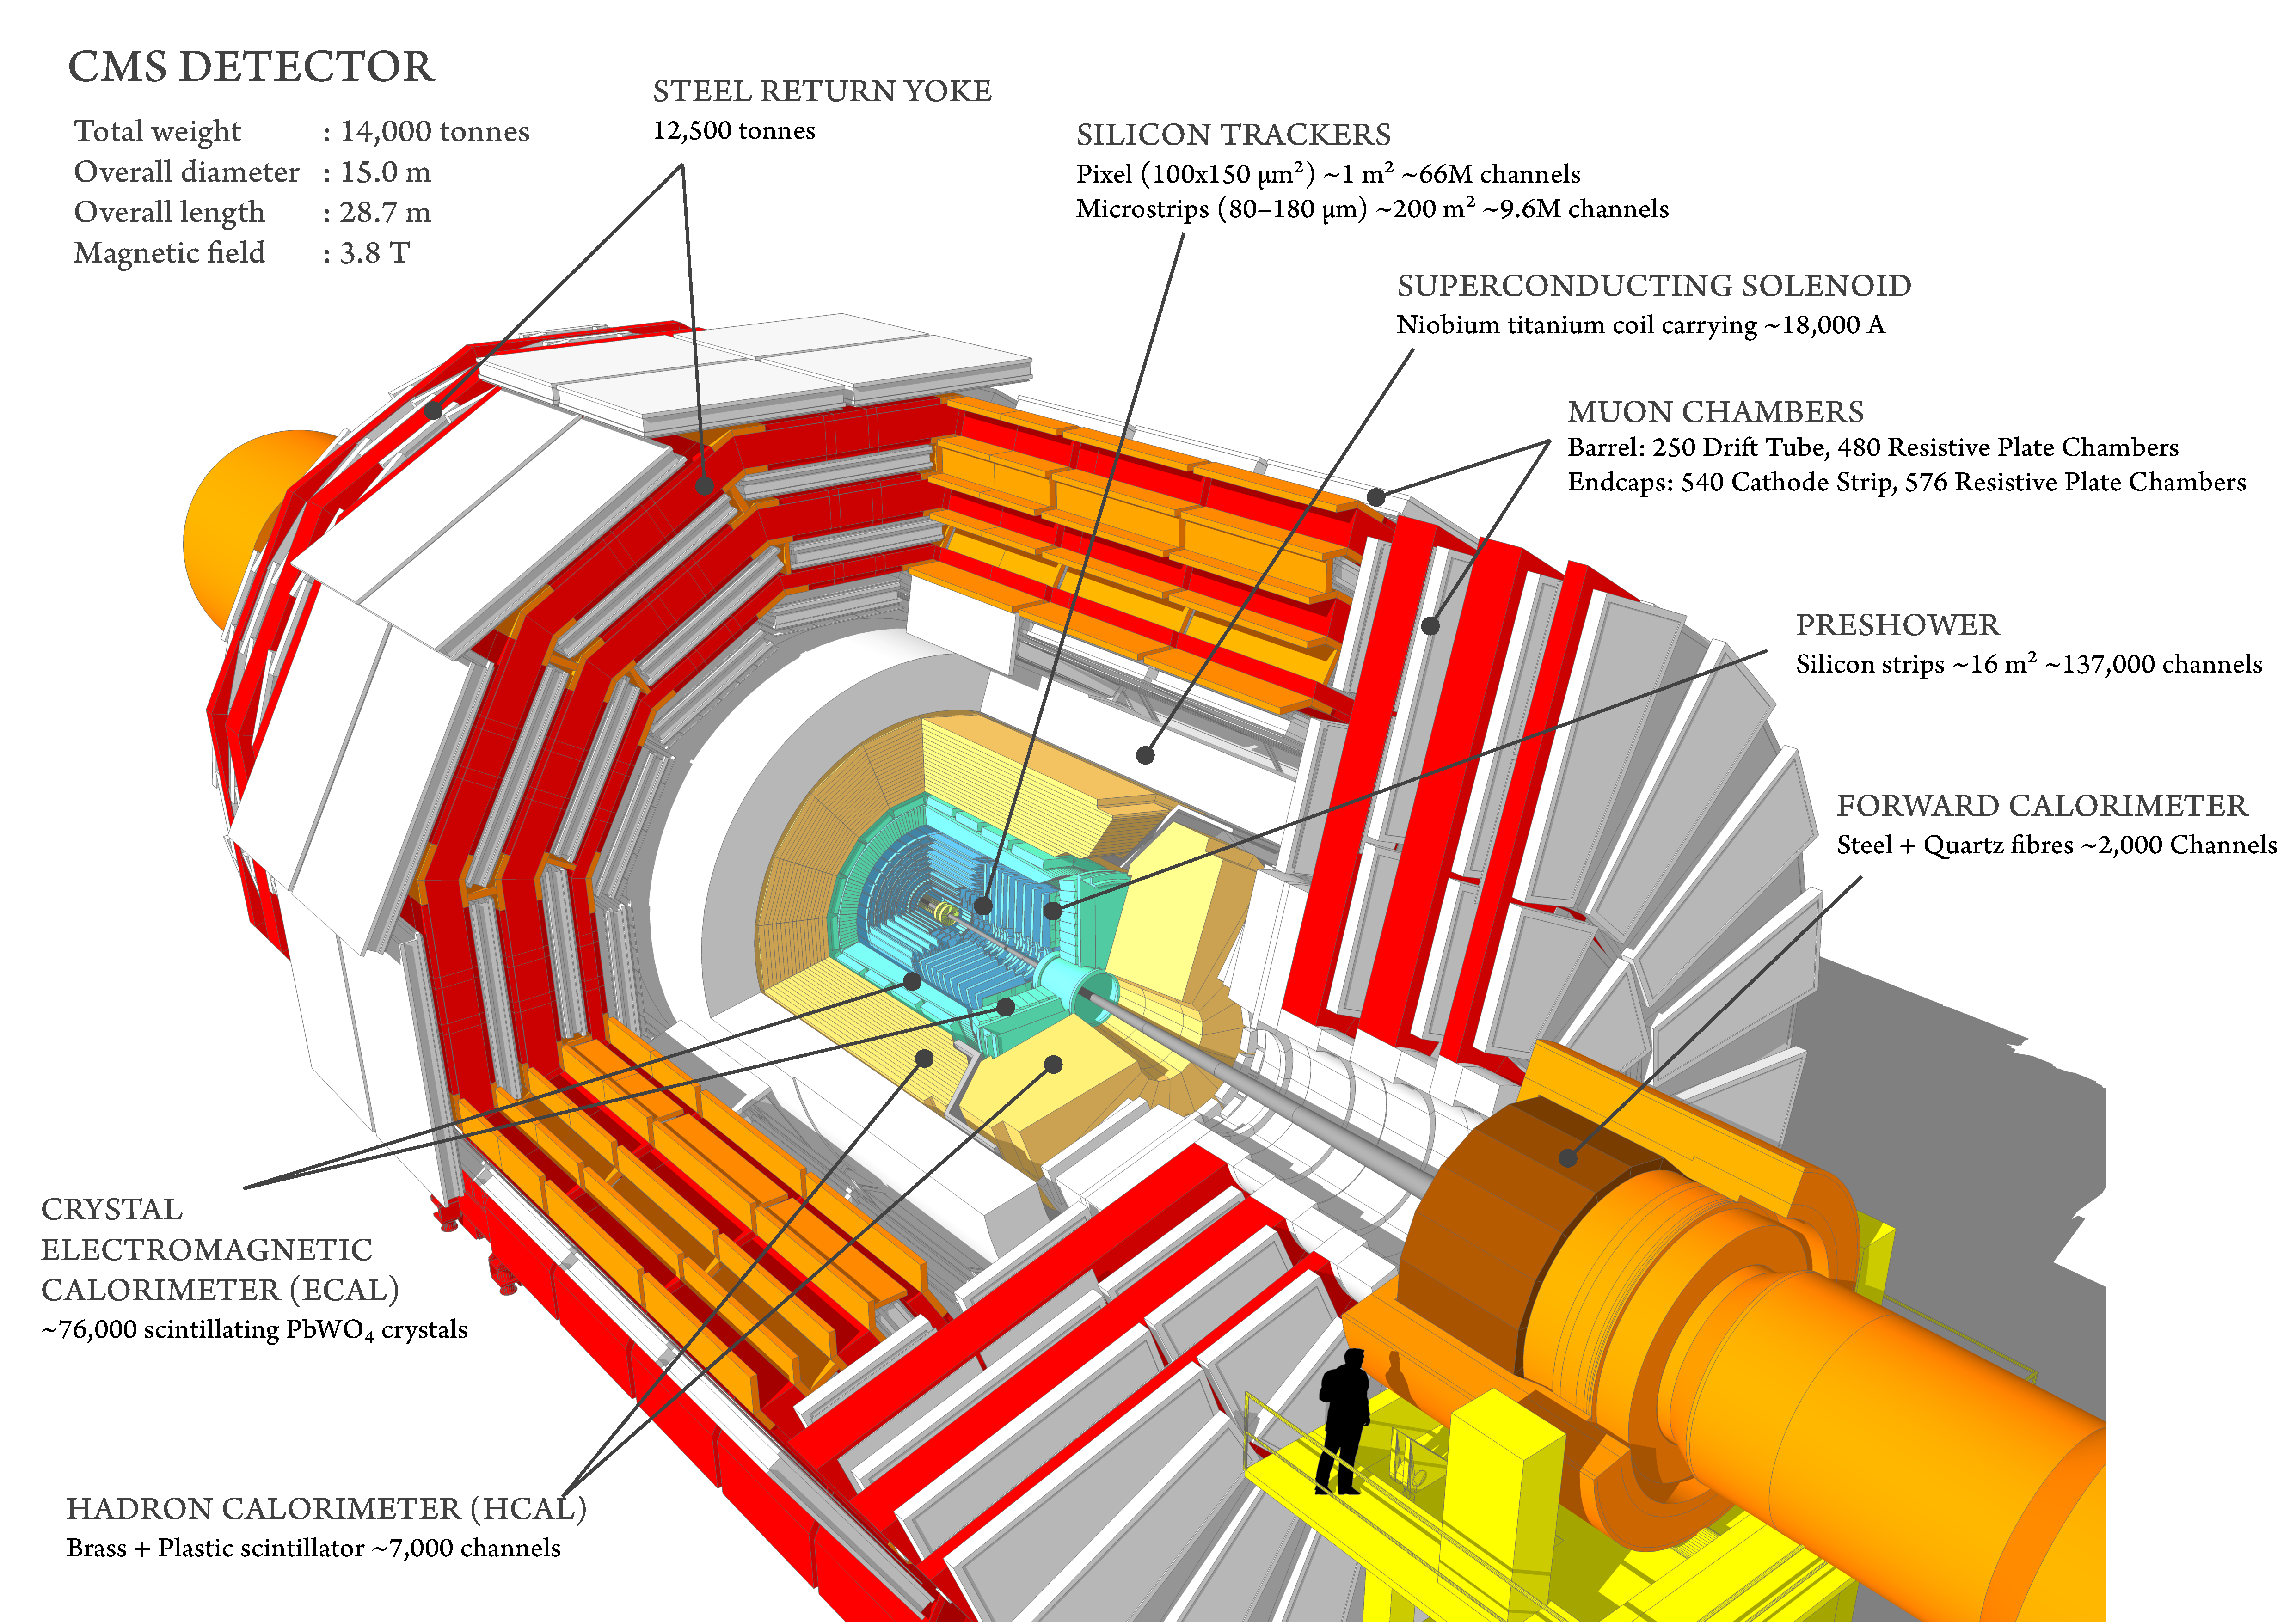
\includegraphics[width=\textwidth]{figures/Part1/Field/CMS}
 \end{minipage}
 \caption{An example of the $\psi^{\prime}\rightarrow\psi\pi^{+}\pi^{-}$ decay recorded by the Mark I detector in the discovery of $\psi$ particle at SLAC~\cite{SLAC-SP-017:1974ind}. A new resonance around 3.1 GeV was reported by this experiment which was later confirmed to be a two-particle bound state consists of charm and anti-charm quarks.}
 \label{fig:JPsi}
 \end{center}
\end{figure}
\chapter{Electroweak Theory}
\label{chap:SM}

Developed in the 1960s, the Glashow–Weinberg–Salam theory of \ac{EW} interaction is regarded by many physicists as the cornerstone of the \ac{SM}. It successfully unified the weak interaction with electromagnetism and postulated the existence of several new particles, all of which were later confirmed by experiments. One of the most important aspects of this theory is the \ew~gauge symmetry, which is discussed in \autoref{sec:Gauge}. The \ew~ symmetry is spontaneously broken through the Higgs mechanism, which is discussed in \autoref{sec:Higgs}. Finally, flavor physics and its connection to the Yukawa interaction is discussed in \autoref{sec:Flavor}. 

\section{Gauge Theory}
\label{sec:Gauge}

Fundamental forces in the \ac{SM} are formulated under a principle known as gauge invariance, where Lagrangian is invariant under local transformations of gauge groups. Taking \ac{QED} as an example, the local symmetry for a Dirac fermion is,

\begin{equation}
\psi\rightarrow e^{i\alpha(x)}\psi,
\end{equation}

where $\alpha(x)$ is a space-time dependent phase angle, hence the name ''local transformation''. The gauge group associated to this symmetry is $U(1)_{EM}$, where the subscript is a shorthand expression for ``electromagnetism''. Under a local $U(1)_{EM}$ rotation, Equation~\ref{eq:Dirac} can be written as:

\begin{equation}
\begin{split}
\label{eq:QEDGauge}
\mathcal{L}&=-\frac{1}{4}F_{\mu\nu}F^{\mu\nu}+ie^{-i\alpha(x)}\bar{\psi}\gamma^{\mu}\partial_{\mu}e^{i\alpha(x)}\psi-m\bar{\psi}\psi-e\bar{\psi}\gamma^{\mu}(A_{\mu}+\delta A_{\mu})\psi\\
&=\mathcal{L}_{Dirac}-\bar{\psi}\gamma^{\mu}\psi\partial_{\mu}\alpha(x)-e\bar{\psi}\gamma^{\mu}\delta A_{\mu}\psi.
\end{split}
\end{equation}

The gauge invariance requires $\delta A_{\mu}=-\frac{1}{e}\partial_{\mu}\alpha(x)$. This means the photon field transforms as:

\begin{equation}
A_{\mu}\rightarrow A_{\mu}-\frac{1}{e}\partial_{\mu}\alpha(x).
\end{equation}

This behavior of the photon field under gauge transformation cancels out the gauge dependency of the free Dirac Lagrangian, which ensures the gauge invariance of the theory. Therefore, vector bosons such as photons also called gauge bosons, and the associated quantum fields are also known as gauge fields. The Dirac Lagrangian can be re-written as,

\begin{equation}
\label{eq:QEDCov}
\mathcal{L}=-\frac{1}{4}F_{\mu\nu}F^{\mu\nu}+i\bar{\psi}\gamma^{\mu}D_{\mu}\psi-m\bar{\psi}\psi,
\end{equation}

where $D_{\mu}=\partial_{\mu}+ieA_{\mu}$ is known as the gauge covariant derivative. 

The mass term associated to the photon field $\frac{1}{2}m^2A_{\mu}A^{\mu}$ is however not gauge invariant as

\begin{equation}
[A_{\mu}-\frac{1}{e}\partial_{\mu}\alpha(x)][A^{\mu}-\frac{1}{e}\partial^{\mu}\alpha(x)]\neq A_{\mu}A^{\mu}.
\end{equation}

Effectively, this means gauge bosons such as photons must be massless in a gauge invariant theory. As a consequence, a new mechanism, known as the Higgs mechanism, is needed to explain the origin of weak boson masses, which is discussed in the following chapter. 

It should be pointed out that gauge symmetry is not a symmetry of nature. Unlike global symmetry that corresponds conserved current~\cite{Noether1918}, gauge symmetry is not physical and can not be measured by experiments. Nevertheless, its existence is necessary to regulate the redundant degree of freedom in the Lagrangian~\cite{SCHWARTZ}. 

\ac{QED} is also known as an abelian gauge theory as the $U(1)$ group operation is commutative. Chinese physicist Yang Chen-Ning and his American colleague Robert Mills at BrookHaven first generalized the concept of gauge invariance to the non-abelian Lie group, proposing what's now known as the Yang-Mills theory in 1954~\cite{Yang:1954ek}. Shortly after this work, Yang and his colleague Tsung-Dao Lee suggested parity might be violated in the weak interaction~\cite{Lee:1956qn}, which was later confirmed by the legendary Wu experiment led by Chien-Shiung Wu~\cite{Wu:1957my}. 

Not long after the Wu experiment, physicists had understood that only left-handed fermions and right-handed anti-fermions are involved in weak charged-current interactions. Moreover, the very existence of weak charged-current forced physicists to consider the interaction between photons and weak mediators. This led to many problems in the weak theory, for example, the exchange of photons in $s$-channel $\textsf{e}^{+}\textsf{e}^{-}\rightarrow\textsf{W}^{+}\textsf{W}^{-}$ would result in divergence at high energy unless there is a new massive neutral particle that mediates the weak interaction. Hints of the weak neutral current and the interplay between electromagnetism and the weak interaction prompted the efforts by physicists to relate these two forces under the framework of non-abelian gauge theory in early 1960s. 

Since fermions with different chiral structures were understood to be treated differently by the weak interaction, it was 
imperative to apply different gauge transformations to left-handed and right-handed fermionic fields. Initial work toward unification was done by American physicist Sheldon Glashow, who proposed the \ew~symmetry in 1961~\cite{Glashow:1961tr}, where $L$ denotes left-handed fields, and Y refers to the quantum number for hypercharge. Under this framework, left-handed components of the Dirac fields are organized into $SU(2)_{L}$ doublet,

\begin{equation}
L_{L}^{j}=\begin{pmatrix}\upnu_{\ell}^{j}\\ \ell^{j}\end{pmatrix}_{L}, Q_{L}^{\prime j}=\begin{pmatrix}q^{\prime j}_{u}\\q^{\prime j}_{d}\end{pmatrix}_{L}, j=1, 2, 3,
\end{equation}

where $\upnu_{\ell}^{j}$, $\ell^{j}$, $q^{\prime j}_{u}$, and $q^{\prime j}_{d}$ correspond to Dirac fields of neutrino, charged-lepton, up-type quark, and down-type quark, respectively. The right-handed components of the Dirac fields are treated as $SU(2)_{L}$ singlet: $\ell_{R}^{j}, u_{R}^{\prime j}, d_{R}^{\prime j}$, where a neutrino term is missing as only left-handed neutrinos have been observed in nature. The index $j$ in both doublets and singlets runs over the fermion generations. The left-handed doublets carry $\frac{1}{2}$ weak isospin charge, denoted by $T$. The third component of $T$, denoted by $T_3$, is $\frac{1}{2}$ for neutrinos and up-type quarks, and -$\frac{1}{2}$ for charged-leptons and down-type quarks in the $SU(2)_{L}$ doublets. All right-handed singlets carries 0 weak isospin charge, which prevents them from participating in the weak interaction. 

The \ew~symmetry introduces the following local gauge transformations:

\begin{equation}
\begin{split}
&\Psi_{L}\rightarrow\textsf{exp}[i\hat{T}_{i}\alpha^{i}(x)+i\frac{\hat{Y}}{2}\beta(x)]\Psi_{L},\\
&\Psi_{R}\rightarrow\textsf{exp}[i\frac{\hat{Y}}{2}\beta(x)]\Psi_{R},
\end{split}
\end{equation}

where $\hat{T}_{i}$ and $\hat{Y}$ denotes generators of the $SU(2)_{L}$ and $U(1)_{Y}$ group, respectively. To preserve gauge invariance, two massless gauge fields $W_{\mu}$ and $B_{\mu}$ are introduced. The corresponding gauge covariant derivative can be written as

\begin{equation}
D_{\mu}=\partial_{\mu}-ig\hat{T}_{i}W_{\mu}^{i}-ig^{\prime}\hat{Y}B_{\mu},
\end{equation}

where $g$ and $g^{\prime}$ coupling strength of the $SU(2)$ and $U(1)$ gauge fields, respectively. A linear combination of the first and second component $W_{\mu}^{i}$ gives rise to the weak charge-current interactions observed in experiments:

\begin{equation}
W^{\pm}_{\mu}=\frac{1}{\sqrt{2}}(W^{1}_{\mu}\mp W^{2}_{\mu}),
\end{equation}

while neutral-current interactions can be constructed by the remaining fields:

\begin{equation}
\label{}
\begin{pmatrix}B_{\mu}\\W_{\mu}^{3}\end{pmatrix}=\begin{pmatrix}\cos\theta_{W}&-\sin\theta_{W}\\\sin\theta_{W}&\cos\theta_{W}\end{pmatrix}\begin{pmatrix}A_{\mu}\\Z_{\mu}\end{pmatrix},
\end{equation}

where $A_{\mu}$ and $Z_{\mu}$ corresponds to the photon and Z boson, respectively, and $g\sin\theta_{W}=g^{\prime}\cos\theta_{W}=e$. The free parameter $\theta_{W}$ is referred to as the week mixing angle, or Weinberg angle, which has to be measured experimentally.

The relation between electric charge, weak isospin, and hyperchage is given by the Gell-Mann-Nishijima formula~\cite{Nakano:1953zz,Gell-Mann:1956iqa}:

\begin{equation}
Q=\frac{Y}{2}+T_{3}.
\end{equation}

The preliminary version of the \ac{EW} theory developed by Glashow didn't collect very good reception initially as all gauge fields in this theory were massless due to gauge invariance. Luckily, physicists didn't have to wait for long as the mechanism proposed by American physicist P. W. Anderson~\cite{Anderson:1963pc} in the following year (1962) had quickly gained attention. Extending on Anderson's work, the theory of symmetry breaking and mass generation was published by Higgs and others in 1964~\cite{PhysRevLett.13.321,PhysRevLett.13.508,PhysRevLett.13.585}, which led to the eventual completion of the \ac{EW} theory in the following years~\cite{Salam:1964ry,Weinberg:1967tq}.

\section{Higgs Mechanism}
\label{sec:Higgs}

\begin{figure}[tbh!]
 \begin{center}
 \begin{tabular}{c}
 \includegraphics[width=0.7\textwidth]{figures/Part1/SM/HiggsPotential}
 \end{tabular}
 \caption{Possible shape of the Higgs potential before symmetry breaking in hot universe (blue) and after symmetry breaking in present universe (yellow).~\cite{universe9040178}}
 \label{fig:HiggsPotential}
 \end{center}
\end{figure}

\section{Flavor Sector}
\label{sec:Flavor}
\chapter{Quantum Chromodynamics}
\label{chap:QCD}

The strong interaction is the fundamental force responsible for binding quarks together into hadrons. It is described by \ac{QCD} which is a gauge theory based on $SU(3)_{C}$ symmetry. One of the key features of \ac{QCD} is the phenomenon known as asymptotic freedom, namely strong force weakens at shorter distance. This property differentiates the strong force with all three other fundamental forces. A brief description of the formulation of \ac{QCD} is given in \autoref{sec:QCD}. Asymptotic freedom predicts that the strong coupling constant, denoted by $\alpha_{S}$, is small at short distance, which allows for perturbative expansion of the probability amplitude. However, the expansion parameter $\alpha_{S}$ at long distance becomes too large and the predictions are therefore no longer reliable. Techniques developed to model \ac{QCD} phenomenon in this regime are collectively known as nonperturbative-\ac{QCD}, which is discussed in \autoref{sec:Collision}.

\section{Formulation of QCD}
\label{sec:QCD}

The theory of strong interaction began taking its current form in 1964 when the quark model was independently proposed by American physicists George Zweig~\cite{Zweig:1964ruk} and his Ph.D. advisor Murray Gell-Mann~\cite{Gell-Mann:1964ewy}. The original objective of this model was to explain the spectrum of new hadrons discovered at rapid speed at the time. In this early version, mesons and baryons were viewed as composite objects formed by spin-$\frac{1}{2}$ particles, named ``quarks'' by Gell-Mann and ``aces'' by Zweig. They came with several quantum charges and three different flavors: $u$, $d$, $s$. The strange quarks in this model had a higher mass, which explained the mass differences between different baryons and mesons.

This model was successful in explaining why protons of same charge were bound together -- they were bound states of more fundamental particles affected by the strong interactions. However, gaps still existed in this model, mostly notably the tension with Fermi-Dirac statistics. It was indicated by this model that the wave function for $\mathrm{\Omega^{-}}$ (sss) should be symmetrical in the interchange of strange quarks. However, the wave function must be antisymmetric because quarks had half spins in this model. Gell-Mann and his collaborations was able resolve this problem in early 1970s by introducing color charges~\cite{Fritzsch:1973pi}. Under this updated framework, each flavor of quark should come with three colors, namely red, green, and blue. The wave functions of hadrons were assumed to be singlets of the gauge group $SU(3)_{C}$. For example, the wave function for $\mathrm{\Omega^{-}}$ baryon can be represented as,

\begin{equation}
(sss)\rightarrow(s_{r}s_{g}s_{b}-s_{g}s_{r}s_{b}+s_{b}s_{r}s_{g}-s_{r}s_{b}s_{g}+s_{g}s_{b}s_{r}-s_{b}s_{g}s_{r}),
\end{equation}

which restored the Fermi-Dirac statistics.  

The force mediators in this theory, known as ``gluons'', are massless vector bosons analogous to photons. They are electrically neutral but carry color charges, which enables the gluon-gluon self-interactions. The dynamics of gluon-gluon and quark-gluon interactions are described by the \ac{QCD} Lagrangian in the following form:

\begin{equation}
\mathcal{L}_{QCD}=-\frac{1}{2}\textsf{tr}G_{\mu\nu}G^{\mu\nu}+\bar{Q}(i\gamma^{\mu}D_{\mu}-m)Q,
\end{equation}

where $Q$ represents colour triplets quark fields $(Q_{r},Q_{g},Q_{b})^{T}$ of the $SU(3)_{C}$ group that run over six different flavors, $m$ corresponds to the mass of quarks. $G_{\mu\nu}$ is known as the gluon field strength tensor given by

\begin{equation}
\label{eq:G}
G_{\mu\nu}^{a}=\partial_{\mu}A_{\nu}^{a}-\partial_{\nu}A_{\mu}^{a}+g_{S}f^{abc}A_{\mu}^{b}A_{\nu}^{c},
\end{equation}

where $g_{S}$ corresponds to the strength of the gauge coupling. The strong coupling constant is also defined as $\alpha_{S}=\frac{g_{S}^2}{4\pi}$, which is analogous to the fine structure constant in \ac{QED}. $t_{a}$ are eight generators of the $SU(3)_{C}$ group, and $A^{a}_{\mu}$ represent eight gauge fields correspond to eight gluons. $f^{abc}$ is the structure constant defined by $[t^{a},t^{b}]=if^{abc}t^{c}$. $D_{\mu}$ is the $SU(3)_{C}$ gauge covariant derivative expresses as:

\begin{equation}
D_{\mu}=\partial_{\mu}-ig_{S}t_{a}A^{a}_{\mu}.
\end{equation}

The non-abelian structure of the $SU(3)_{C}$ group implies that the third term in Equation~\ref{eq:G} is nonzero as  $SU(3)_{C}$ generators do not commute with each other. This leads to the trilinear and quartic gluon self-interactions when expanding the kinetic (first) term of the \ac{QCD} Lagrangian. 

In parallel to the development of the quark model, Feynman proposed a model to explain the behavior of deep inelastic scatterings~\cite{Feynman:1969wa}. In this model, Feynman postulated that protons are made of point-like constituents called ``partons'', and they behave like free particles at high momentum transfer. Since the de Broglie wavelength~\cite{deBroglie:1924ldk} is given by 

\begin{equation}
\lambda=\frac{h}{p}, 
\end{equation}

a high momentum transfer corresponds to smaller wavelength and consequently better experimental resolution at distance scale. The parton model was an immediate success as it was able to predict the short distance ``Bjorken scaling'' effects of the strong interaction at a very good precision~\cite{Bjorken:1969ja}. Despite the success at describing experimental data, the parton model was still viewed as a phenomenological approximation as Feynman provided no microscopic description of the strong interactions. It was later recognized that partons were matched to quarks, anti-quarks, and gluons within the nucleons.

Two years after Dutch physicist Gerard 't Hooft showed that non-abelian gauge theories were renormalizable~\cite{tHooft:1971akt}, major breakthrough came in 1973 when American physicists H. D. Politzer, David Gross, and Frank Wilczek~\cite{Gross:1973id,Politzer:1973fx} investigated the scale dependency of the strong coupling const $\alpha_{S}$. 't Hooft also arrived at similar results himself sometime earlier but he didn't publish his work. At one-loop precision, the $\alpha_{S}(\mu^2)$ is given by:

\begin{equation}
\label{eq:af}
\alpha_{S}(\mu^2)=\frac{\alpha_{S}(\mu_{R}^2)}{1+\beta_{0}\alpha_{S}(\mu_{R}^2)\textsf{ln}(\frac{\mu^2}{\mu_{R}^2})}
\end{equation}

where $\mu$ is the energy scale, $\mu_{R}$ is known as the renormalization scale, which corresponds to the initial energy scale at which $\alpha_{S}$ is evaluated. $\beta_{0}=(33-2n_{f})/12\pi$ is a constant that depends on the number quark flavors that can be considered massless. Even though the strong coupling constant can not be predicted from the first principle, Equation~\ref{eq:af} allows physicists to predict its value at an energy scale $\mu$ using its measured value at a different scale $\mu_{R}$.

Equation~\ref{eq:af} also reveals that when $n_{f}~<16$, the strength of the strong coupling decreases as energy increases. In other words, quarks and gluons behave like free particles at very short distance. The discovery of this property, known as ``asymptotic freedom'', by Politzer, Gross, and Wilczek brought the \ac{SM} to its current formulation. Since then it has withstood the test of numerous measurements conducted at various experiments across a wide range of energy spectrum. A summary of recent measurements of $\alpha_{S}$ is given in Figure~\ref{fig:alphaS}.

\begin{figure}[tbh!]
 \begin{center}
 \begin{tabular}{c}
 \includegraphics[width=0.8\textwidth]{figures/Part1/QCD/alphaS}
 \end{tabular}
 \caption{The strong coupling constant $\alpha_{S}$ as a function of energy scale $Q$. Measurements done by \ac{CMS}, \ac{ATLAS} and other experiments were shown in points with uncertainty bars. Theoretical predictions based on the renormalization group equation are shown in the dashed line.~\cite{cms:twiki}}
 \label{fig:alphaS}
 \end{center}
\end{figure}

\section{Nonperturbative QCD and Hadron Collisions}
\label{sec:Collision}

Perturbation theory is by far the best developed tool for calculating scattering cross-sections from the first principle. Despite being very successful, its predicting power becomes increasingly worse as the expansion parameter grows larger. As discussed earlier, the strong interaction grows stronger very rapidly at low energy which invalidates the perturbative expansions of parameter $\alpha_{S}$. The transition from perturbative \ac{QCD} regime to nonperturbative \ac{QCD} regime is illustrated in Figure~\ref{fig:pQCD}. The energy scales at which $\alpha_{S}$ diverges is known as $\mathrm{\Lambda}_{QCD}$, which is roughly $\mathcal{O}$(300 MeV)~\cite{Deur:2016tte}.

\begin{figure}[tbh!]
 \begin{center}
 \begin{tabular}{c}
 \includegraphics[width=0.7\textwidth]{figures/Part1/QCD/pQCD}
 \end{tabular}
 \caption{The strong coupling constant $\alpha_{S}$ as a function of distance scale. Experimental determinations are shown in filled points while theoretical predictions are shown in the red line. The dashed blue band separates the regime where perturbative approach is still valid with the regime where perturbative approach is no longer valid.~\cite{Messchendorp:2013ysj}}
 \label{fig:pQCD}
 \end{center}
\end{figure}

The high energy hadron collisions involve phenomena occurred on a wide range of distance or energy scales. The process that carries the highest momentum transfer in a collision event, referred to as ``hard scattering'', typically involves short-distance quark-gluon interactions where production cross-sections calculated by perturbative \ac{QCD} are still valid. It is therefore critically important to separate the hard scattering from those long-distance effects in order to apply the perturbative \ac{QCD} in any cross-section calculations. This is achieved through the so called \ac{QCD} ``factorization theorem''~\cite{Collins:1989gx} whereby scattering cross-sections are decomposed as the product of several ``factors''. Each of these factors involves phenomena occurred on a single distance scale. An illustration of the factorization is shown in Figure~\ref{fig:factorization}.

\begin{figure}[tbh!]
 \begin{center}
 \begin{tabular}{c}
 \includegraphics[width=0.9\textwidth]{figures/Part1/QCD/factorization}
 \end{tabular}
 \caption{Illustration of the physics of proton-proton collisions. The two incoming protons are shown on the left. The \ac{PDF} characterizes the properties the two partons that participate in hard interaction. The short-distance physics is handled by the perturbative \ac{QCD} which is represented with the rectangular box. The outgoing partons undergoes hadronization which is described by the fragmentation function.~\cite{Huston:fact}}
 \label{fig:factorization}
 \end{center}
\end{figure}

Protons are made of two up quarks and one down quark, known as the ``valence quarks''. Since the total mass of the three valence quarks is much smaller than the mass of a proton, most of the proton mass manifests as strong interactions within the nucleons. The mediators of the these interactions -- the gluons can also spawn a pair of quark and anti-quark, forming part of the proton internal structure known as the ``proton sea''. Therefore, it is possible for strange, charm or even bottom quarks to initiate a hard scattering,  and the three-quark view of the proton is largely ineffective in the context of hadron collisions. Moreover, before the initial state of the hard scattering reveals itself, the quarks and gluons inside the proton maintain a relatively large distance between each other, exchanging largely nonperturbative effects. This makes it virtually impossible to predict how the proton is structured from the first principle. Instead, a phonological approach, inspiration by Feynman's parton mode, is used to describe the proton internal structure. Under this approach, protons are seen as streams of quarks and gluons, collectively known as partons. These partons are considered collinear with the proton movement and each carry a fraction of the total proton momentum. The probability of a specific parton that carries x fraction of the proton moment is given by the \ac{PDF}.


In high-energy collisions involving hadrons, the large-momentum scattering is under- stood as the interaction between fundamental hadron constituents, called partons. In such collisions, the production cross section for any process can be calculated using a master formula known as QCD factorization theorem, which postulates the full factorization between short-distance (i.e. non-perturbative) and long-distance (i.e. perturbative) physics. The scale that defines the boundary between short- and long-distance dynamics is known as factorization scale, and is indicated with  According to the factorization theorem, the cross section for a proton-proton inter- action of the kind can be expressed as the convolution of the partonic cross section with the parton distribution functions (PDFs) of the proton 

In high-energy collisions involving hadrons, the large-momentum scattering is under- stood as the interaction between fundamental hadron constituents, called partons. In such collisions, the production cross section for any process can be calculated using a master formula known as QCD factorization theorem, which postulates the full factorization between short-distance (i.e. non-perturbative) and long-distance (i.e. perturbative) physics. The scale that defines the boundary between short- and long-distance dynamics is known as factorization scale, and is indicated with  According to the factorization theorem, the cross section for a proton-proton inter- action of the kind can be expressed as the convolution of the partonic cross section with the parton distribution functions (PDFs) of the proton 

In high-energy collisions involving hadrons, the large-momentum scattering is under- stood as the interaction between fundamental hadron constituents, called partons. In such collisions, the production cross section for any process can be calculated using a master formula known as QCD factorization theorem, which postulates the full factorization between short-distance (i.e. non-perturbative) and long-distance (i.e. perturbative) physics. The scale that defines the boundary between short- and long-distance dynamics is known as factorization scale, and is indicated with  According to the factorization theorem, the cross section for a proton-proton inter- action of the kind can be expressed as the convolution of the partonic cross section with the parton distribution functions (PDFs) of the proton 
\chapter{Beyond the Standard Model}
\label{chap:BSM}

\section{Neutrino Oscillation and SM Extensions}

\section{Leptoquark Model}
\chapter{Effective Field Theory}

\section{Standard Model EFT}

\section{Low Energy EFT}

